%%% NUMBERING OF FIGURES %%%

\subsection{Methodological development and implementation}
\label{PocketVec_MethDevAndImp}

It is known that similar proteins tend to bind similar ligands\cite{klabunde_chemogenomic_2007}, a principle behind many drug discovery projects\cite{sydow_advances_2019, keiser_relating_2007, falaguera_illuminating_2023}. We re-assessed the validity of this principle and found that, indeed, proteins from the same family (e.g. GPCRs) tend to have more similar active compounds than proteins from different families (Fig \ref{PocketVec_FigS1}). However, globally dissimilar proteins showing similar physicochemical and shape properties in their druggable pockets may still bind with similar ligands, which reasonably translates into a more precise and general form of the chemogenomics principle: similar pockets bind similar ligands\cite{gao_comprehensive_2013}. PocketVec builds on this observation to generate novel vector-type descriptors for characterizing protein small molecule binding pockets. 

Instead of directly characterizing the shape and physicochemical environment of the protein
cavities, we rely on a predefined set of small molecules and assess their potential binding to a
given pocket. More specifically, given a three-dimensional protein structure, we first identify
possible druggable pockets and we then use computational docking strategies to assess the
potential binding of the small molecules. The resulting docking scores are then translated into
rankings, which are finally stored in a vector-type format. In this way, each bit of the vector
represents the ranking of a predefined molecule, illustrating how good it binds with the pocket of
interest compared to all other molecules (Fig \ref{PocketVec_Fig1}a). While the idea is conceptually pretty straightforward, its implementation requires a thorough assessment of the set of used molecules, the docking methodology and the benchmark strategy. The following sections describe our effort to evaluate and optimize each step of the procedure.

\phantomsection
\subsubsection{Selection of the methodological pipeline}

To find the optimal set of compounds to develop our binding pocket descriptors, we tested two different types of molecules. On the one hand, we used the Glide chemically diverse collection of fragments\cite{friesner_glide_2004, halgren_glide_2004}, containing 667 compounds with molecular weights in the 50-200 g·mol\textsuperscript{-1} range (Fig \ref{PocketVec_FigS2}). Additionally, we also selected 1,000 lead-like molecules (LLM) from the MOE v2019.01 dataset (Chemical Computing Group, Montreal, Canada), exhibiting molecular weights in the 200-450 g·mol\textsuperscript{-1} range (Fig \ref{PocketVec_FigS2}).

We also assessed the performance of two well-established small molecule docking strategies. More specifically, we used rDock\cite{ruiz-carmona_rdock_2014} and SMINA\cite{koes_lessons_2013} to run rigid and flexible docking calculations, respectively, under the default parameters.

Finally, to determine the best combination of small molecules and docking methods we relied on ProSPECCTs, a collection of datasets aimed at evaluating the performance of pocket comparison approaches (including pocket descriptors) in a wide range of distinct scenarios\cite{ehrt_benchmark_2018}. In brief, ProSPECCTs comprises 10 datasets consisting of protein-ligand binding site pairs classified as either similar or dissimilar according to various criteria, including pairs of different structures of the same proteins, proteins harboring artificial mutations in their binding pockets or pairs of unrelated proteins that are able to bind chemically similar ligands (Fig \ref{PocketVec_FigS3}).

Please, see the \hyperref[PocketVec_Methods]{Methods} section for a more detailed description of the methodological pipeline.

\phantomsection
\subsubsection{PocketVec parameter selection and benchmark}

For each ProSPECCTs dataset, we generated PocketVec descriptors for all ligand-defined protein binding sites, and evaluated pocket similarity on the basis of pairwise cosine distances between PocketVec descriptors: the lower the PocketVec distance, the higher the pocket similarity. 

First, we obtained results for all possible combinations of docking strategies (rDock--rigid docking and SMINA--flexible docking) and compound collections (1,000 lead-like molecules and 667 fragments). We observed that, in general, the use of LLM and rDock rigid docking provided better results than other combinations (Fig \ref{PocketVec_FigS4}). Positive docking scores (i.e. molecules that could not be accommodated in the binding pocket, see \hyperref[PocketVec_Methods]{Methods} for further details) leading to outlier rankings were rare with fragments but more frequent when using LLM (\textasciitilde35\% of structures had at least one outlier molecule in the rDock--LLM (1,000) combination, Fig \ref{PocketVec_FigS5}). Thus, LLM showed a superior discriminative power with respect to the size of the pocket and, overall, provided higher ranking diversity among all ProSPECCTs pockets (Fig \ref{PocketVec_FigS6}). In fact, we observed how LLM occupied a larger fraction of the binding sites than fragments, while rigid docking might have removed the noise created by similar rankings of the same ligand in different conformations, overall conferring a superior discrimination capacity to the rDock--LLM combination.

Our benchmarks also revealed that some molecules were systematically ranked as very weak binders and were thus not informative for the assessment of pocket similarity. Indeed, we realized that the use of \textasciitilde100-200 molecules was often sufficient to get competitive performances in most datasets. In order to optimize the set of predefined molecules to derive pocket descriptors, we selected those LLM and fragments presenting high ranking diversity across all ProSPECCTs datasets (see \hyperref[PocketVec_Methods]{Methods}). In brief, we calculated the Shannon’s entropy for each molecule within each dataset and, after intra-dataset normalization, we assigned each molecule an averaged entropy value, which enabled us to prioritize those molecules presenting high ranking diversity (high entropy). Indeed, performances obtained in ProSPECCTs datasets by the 128 most diverse molecules were fairly similar to the original ones using complete sets of compounds (Fig \ref{PocketVec_Fig1}b, Fig \ref{PocketVec_FigS7}). Reducing the number of docked molecules (from 1,000/667 to 128) enabled a shorter length of the descriptor, now compatible with other small molecule and biological descriptors derived in the group\cite{fernandez-torras_integrating_2022, duran-frigola_extending_2020, bertoni_bioactivity_2021}, and alleviated the overall computational cost of the methodology. An illustrated example of low- and high-entropy lead-like molecules is shown in Fig \ref{PocketVec_Fig1}c.

Overall, and in view of the benchmark results, we established that the use of rigid docking (rDock) and 128 LLM was the standard and optimal methodology to generate PocketVec descriptors. All results presented along the rest of the manuscript were derived following this strategy. The selected LLM are shown in Fig \ref{PocketVec_FigS8_v2} and can also be found in our \hl{GitLab repository} in SMILES and SDF format, together with their commercial names. 

%%%%%%%%%%%%%%%%
%%% FIGURE 1 %%%
%%%%%%%%%%%%%%%%


\begin{figure}[htbp]
  \centering
  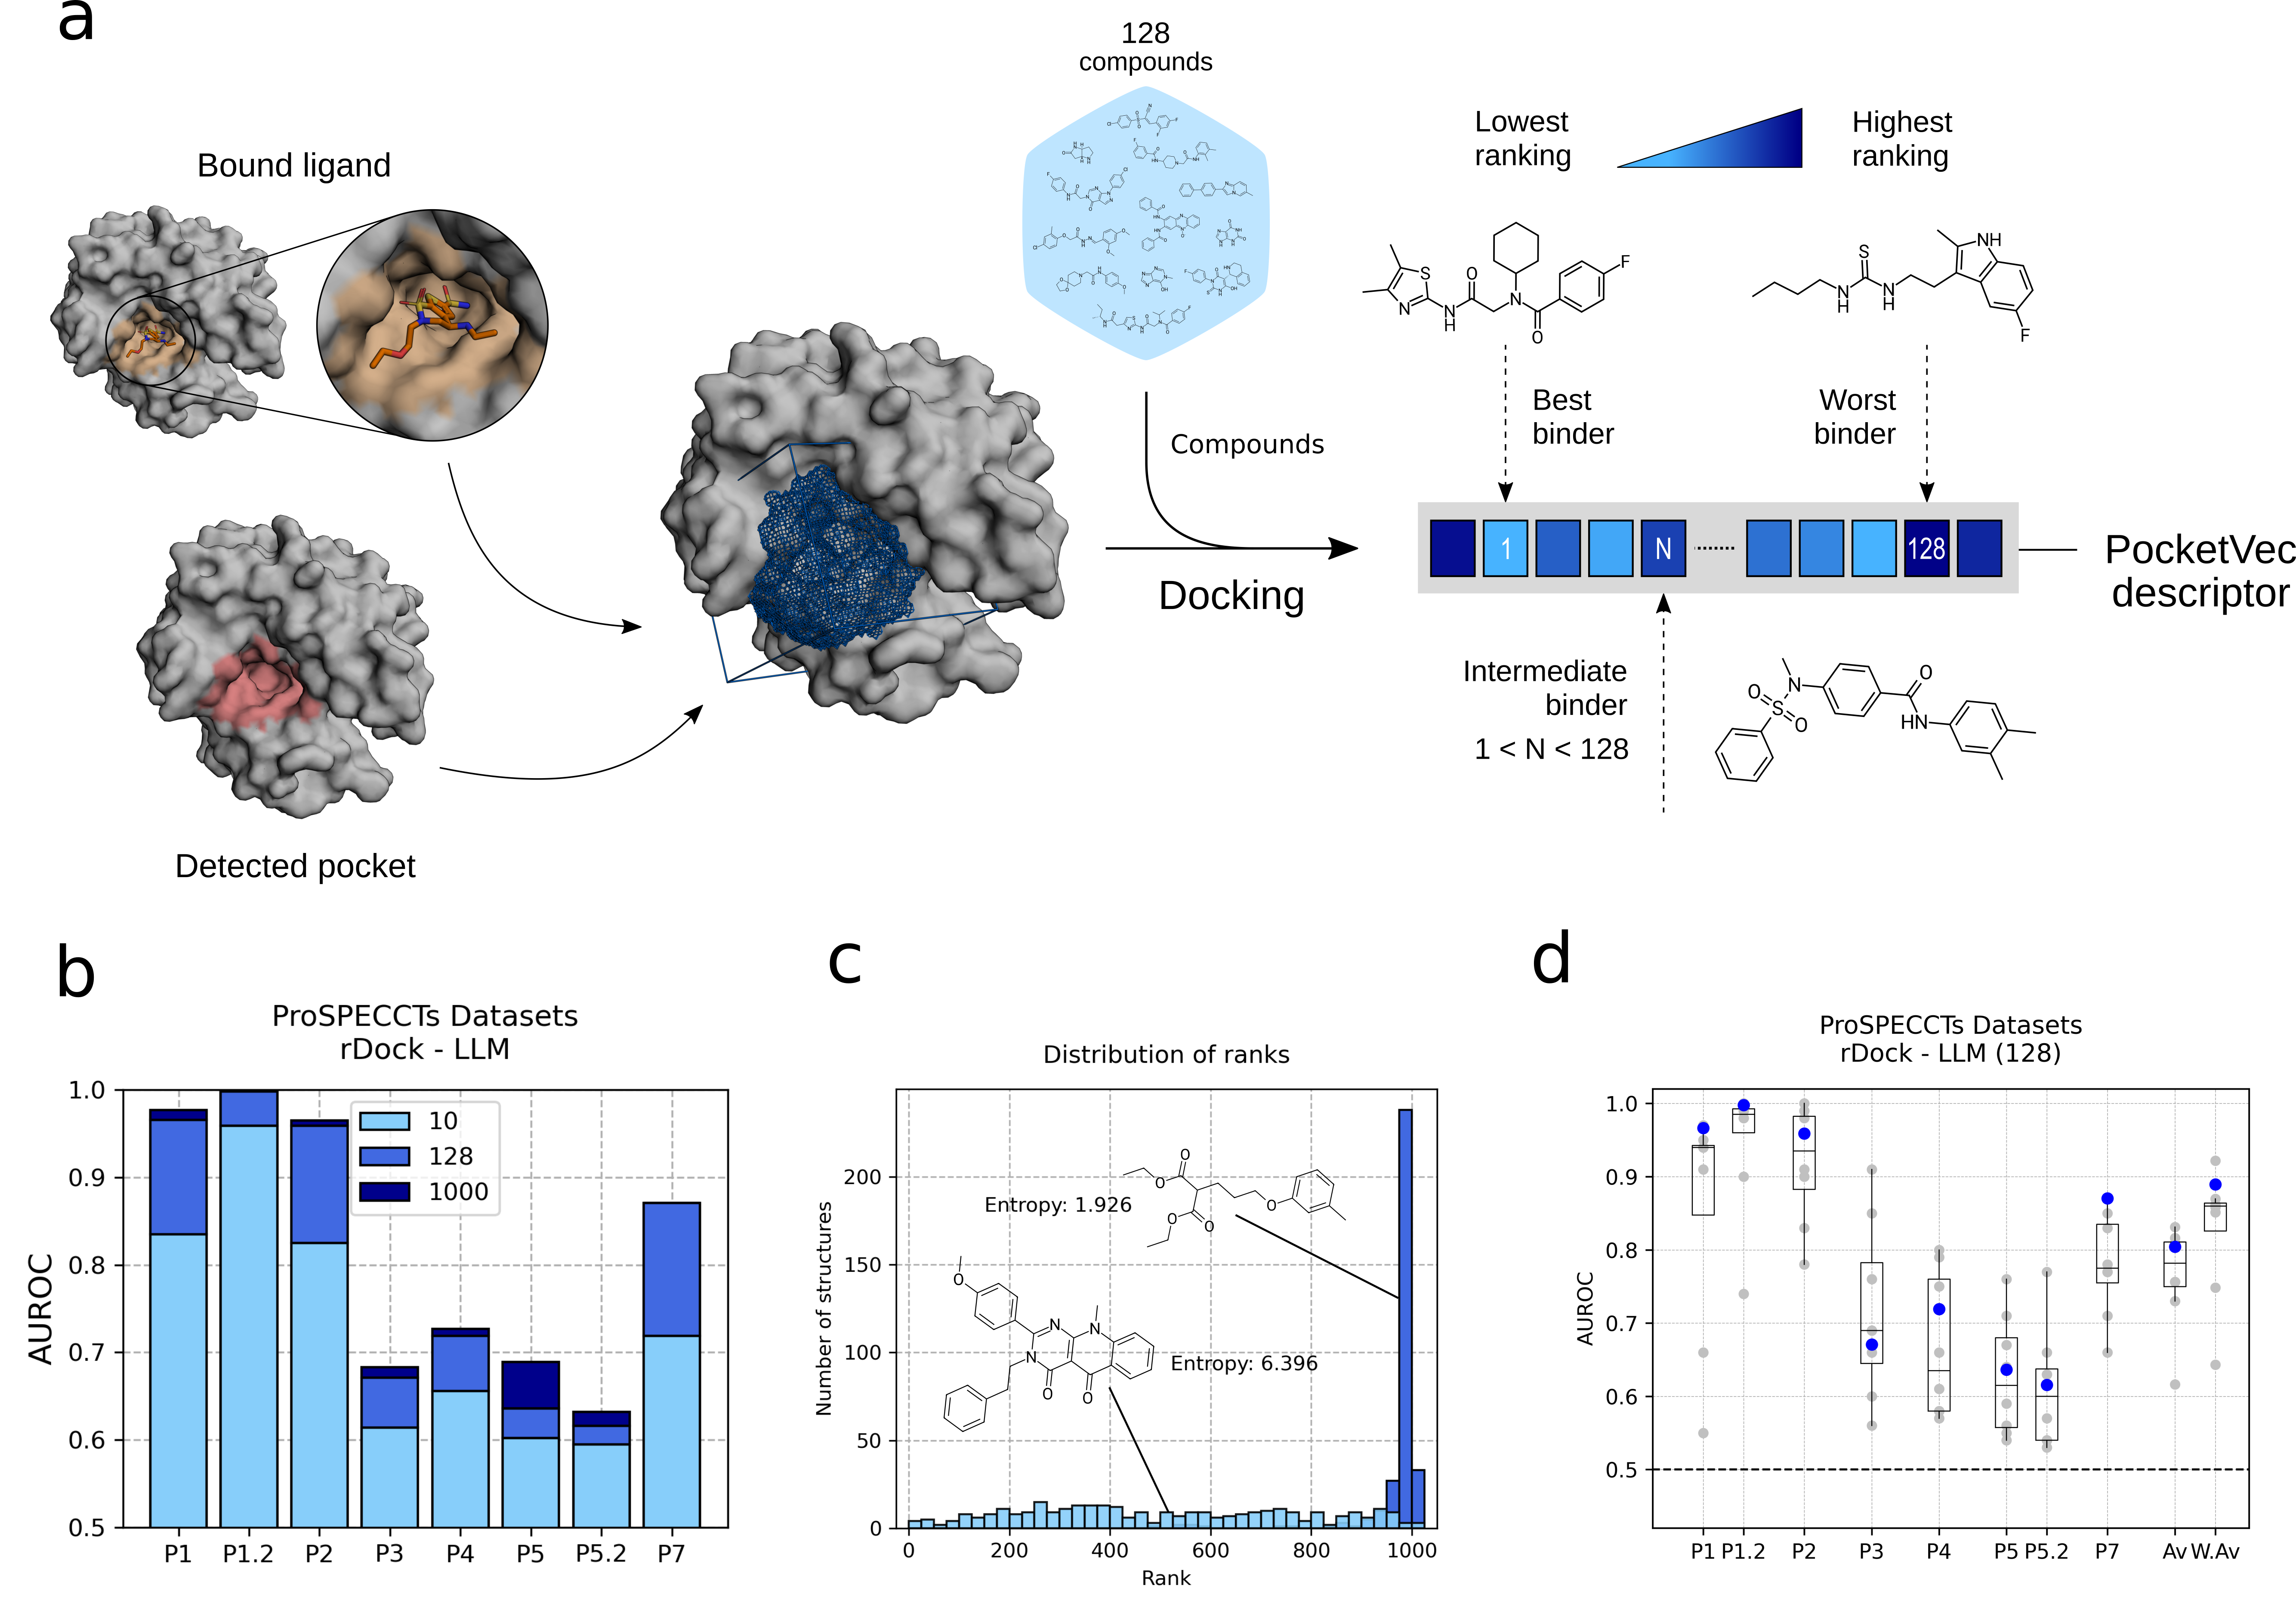
\includegraphics[width=\linewidth]{figures/PocketVec/Main/Fig1.png} 
  \caption{
    \textbf{PocketVec methodological pipeline and benchmark results.} 
    \textbf{a)} Given a 3D protein structure, binding site locations are established by the presence of bound ligands or by means of pocket detection algorithms. A predefined set of compounds (128 lead-like molecules in the standard PocketVec pipeline) is docked against the pocket of interest. The corresponding docking scores are then converted into rankings and stored in a vector-type format that serves to characterize the pocket. We refer to those vectors as PocketVec descriptors.
    \textbf{b)} Bars indicating the performance (AUROC, y-axis) of our descriptors generated with a varying number of predefined molecules among ProSPECCTs datasets (x-axis, P6 and P6.2 not included. For further details, please see Online Methods). Bar color indicates the number of predefined compounds (10, 128 and the complete set of 1,000 lead-like molecules, sorted by entropy). These results correspond to the rigid docking (rDock) and LLM combination. All the other combinations with all possible numbers of predefined compounds (from 1 to complete sets) are shown in Fig \ref{PocketVec_FigS7}.
    \textbf{c)} Predefined molecules with high and low entropy. The histograms depict the distribution (y-axis) of rankings (x-axis, bin width: 25) for the highest (sky blue) and lowest (dark blue) entropy lead-like molecules in ProSPECCTs P1. Their chemical structures are shown together with the corresponding entropy values.
    \textbf{d)} Performances (AUROC, y-axis) of distinct pocket descriptors among ProSPECCTs datasets (x-axis, P6 and P6.2 not included). Gray dots represent the individual performances of existing strategies to derive pocket descriptors (see Table \ref{PocketVec_TableS1}). Box plots indicate median (middle line), 25th, 75th percentile (box), and max and min value within the 1.5*25th and 1.5*75th percentile range (whiskers). Blue dots indicate the performance of PocketVec descriptors (128 LLM and rDock rigid docking). Av. values represent the average performance among ProSPECCTs datasets for each individual method and W. Av. values weight the average value according to the number of pairs within each dataset.
  }
  \label{PocketVec_Fig1}
\end{figure}
